\cotefile{149}

\scanpage{130}
se ramène à celle des hom composants.

À ce sujet, sous réserve de vérifications, je présume

$1^\circ)$ que l'hom $\mathcal E_{\tilde U_x}^{\bar L}\longrightarrow\mathcal E_U^{\bar L}$ est \uline{injectif}

--- ou ce qui revient au $=$, que sa partie géométrique
\diagram{\begin{tikzcd}[column sep=large,row sep=small]
\mathcal E_{\tilde U_x/K}^{\bar L}\arrow[r]\arrow[d,equal] & \pi_{U/K}^{\bar L}\\
I_x\simeq T^{(I(x))} &
\end{tikzcd}}
\margin{les deux lettres $I$ ne sont pas les mêmes}
est \uline{injective}.

\margin{C'est visiblement \uline{faux} \inserted{\uline{``en général''}} pour $\operatorname{card}I(x)\ne1$ comme on voit en \unsure{passant} à un autre modèle $X'$ déduit de $X$ en y faisant éclater un pt de $D$\ldots\ Mais y a-t-il un modèle ``minimal'' $X\supset U$, et pour un tel modèle \unsure{a-t-on} l'injectivité ???}

$2^\circ)$ que \deleted{l'hom} lorsque le corps résiduel de $V$ est alg $/K$ (i.e. $V$ correspondant à un pt de $\mathfrak X_{L/K}$ de dim zéro), alors l'hom
\[
 \mathcal E_{\tilde\eta}^{\bar L}=N_V\longrightarrow\mathcal E_{\tilde U_x}^{\bar L}
\]
\deleted{est injectif} \inserted{\unsure{a} une image} \deleted{surjectif} \inserted{ouverte} --- ce qui revient ici (puisque $k(V)$ \deleted{alg} \inserted{fini} sur $k(x)$ donc $\mathcal E_{k(V)}=N_V/I_V\hookrightarrow\mathcal E_{k(x)}$ \inserted{(sous-groupe ouv.)} $\simeq N_x/I_x$), que la partie géométrique
\[
 I_V\longrightarrow I_x=T^{I(x)}
\]
\deleted{est injective} \deleted{\inserted{\unsure{surjective}}} \inserted{a une image ouverte} \deleted{--- \unsure{je pense que} \illegible{3} \unsure{à un sous-groupe ouvert}.} \inserted{--- sans doute est-elle $=$ surjective.}

À noter que \unsure{la} question $2^\circ$ est purement
\margin{129}

\scanpage{131}
\mspage{65}
locale autour de $x$ --- elle doit être essentiellement ``triviale'', que ma présomption s'avère vraie ou fausse --- par contre $1^\circ)$ est une question de nature globale sur $U$, et sans doute d'\deleted{\unsure{autre}} aucune façon triviale.

\deleted{Avant de \unsure{co|ce}} La validité de ces énoncés \deleted{signifierait} \inserted{impliquerait} donc, pour les sections de $\mathcal E_U^{\bar L}$ sur $\mathcal E_K^{\bar L}$ associées à un anneau de valuation de $L/K$, \inserted{de corps résiduel $K$} que l'image de $\mathcal E_K^{\bar L}$ doit normaliser un \deleted{$I_x$} sous-groupe $\unsure{\Delta_x|\bar\Delta_x}\simeq T^{I(x)}$ de $\pi_{L/K}^{\bar L}$, qui est non trivial si la valuation n'a pas de centre sur $U$, i.e. si la section n'est pas associée à un pt $K$-rationnel de $U$, ce qui est justement dans le sens des conjectures (qui pouvaient d'abord sembler hâtives !) du § $2$.

Avant de me tourner vers l'étude des questions $1^\circ)$ et $2^\circ)$ (et \inserted{aussi} des questions de normalisation et de centralisation soulevées
\margin{130}

\scanpage{132}

précédemment à propos des $N_V,I_V\ldots.$), je vais regarder d'un peu plus près l'allure des sous-groupes $I_x\subset\unsure{\pi|\mathcal E}_{L/K}^{\bar L}$, ou \deleted{\unsure{associés}} plutôt, des classes de \inserted{$\pi$-}conjugaison de tels sous-groupes) associés aux $x\in X\setminus U$, \inserted{pour $x$ variable,} et me convaincre du caractère intrinsèque de ces groupes, indépendamment du choix du modèle $X$ (mais ceci est évident, si on admet ce qu'on vient d'\unsure{énoncer|annoncer} --- que ce sont justement, à sous-groupes ouverts près \deleted{\unsure{tout}} au plus, les images des $I_V$, pour $V\deleted{\unsure{\to}}\inserted{\in}\mathfrak X_{L/K}$ n'ayant pas \inserted{de} centre dans $\deleted{X\setminus U}U\ldots$)

\deleted{Considérons d'abord les}

Soit $J$ une partie de l'ens. fini $I$, et soit
\[
D_J^*=\{x\in X\mid I(x)=J\}
=\overbrace{\bigcap_{j\in J}D_j}^{\Delta_J}-\bigcup_{i\in I\setminus J}\Delta_J\cap D_i
\]
de sorte que
\[
D_{\{i\}}=D_i\setminus\left(\bigcup_{j\ne i}\unsure{D_i\cap D_j}\right).
\]
Si $d=\operatorname{card}J$, on voit que $D_J\subset X$ est \inserted{régulier,} de codim $d$ en chacun de ses points (mais bien sûr, il peut être $\phi$). Si on appelle ``simplexe'' une partie $J\subset I$

\margin{il vaut mieux définir $D_J$ comme \uline{sous-schéma} comme $\bigcap_{j\in J}D_j$ (36), et définir son \uline{\unsure{support|sous-ouvert}} comme $\{x\in X\mid I(x)=J\}$}

\margin{131}

\scanpage{133}
\mspage{66}

telle que $D_J\ne\phi$, \inserted{(i.e. $\bar D_J=\bigcap_{j\in J}D_j$ soit $\ne\phi$)} on trouve sur $I$ une structure de \deleted{\unsure{solide}} \inserted{maquette} simpliciale --- quelle est sa signification topologique? Les composantes connexes correspondent comp. connexes de $D=X\setminus U$ --- ou encore : celles de $\deleted{\unsure{U_\infty}}\hat X\setminus D$, où $\hat X$ est le \inserted{l'ombre} complété de $X$ le long de $D$ --- et $\hat X\setminus D$ a un caractère invariant p.r. à la ``\unsure{compactification|complétification}'' choisie $X$ de $U$. S'il était vrai que les $D_J$ \inserted{non vides} sont $\infty$-connexes (ce qui bien sûr n'est \uline{pas} le cas, sauf pour $D_J$ réduit à un point!) on pourrait penser que la topologie de notre \deleted{\unsure{solide}} \inserted{maquette} simpliciale exprime le type d'homotopie de $U_\infty$.

Considérons maintenant le ``localisé'' \deleted{\unsure{de}} (au sens des ombres, ou en un sens étale convenable) de $X$ le long de $D_J$, soit $\deleted{\unsure{\hat X_J}}X_J$, et soit $U_J$ \inserted{$=X_J\setminus D_J$} la trace de $U_\xi$ sur $X_J$. Considérons $\mathcal E_{U_J}$ (de façon précise, $\mathcal E_U^{\bar L}$, si on localise \deleted{p.r. à} étalement), on aura une suite exacte
\[
\tag{37}
T^J\unsure{\hookrightarrow|\to}\mathcal E_{U_J}^{\bar L}\longrightarrow\mathcal E_{D_J}^{\deleted{\unsure{\tilde D_J}}}\longrightarrow1
\]
\margin{plutôt}
--- de façon précise, choisissant un rev. universel $\tilde D_J$ de $D_J$, on trouvera un rev. universel \inserted{par image inverse} $\tilde X_J$ de $X_J$, d'où d'ailleurs $\tilde U_J$ et $\tilde U_J\longrightarrow U$ ; \deleted{\unsure{et on}} on désigne par $\tilde L_J$ le corps des fonctions de $\tilde X_J\unsure{\mathrel{\cdot-}}\tilde U_J$, c'est une ext. \inserted{alg sép} de $L$, et

\margin{il vaut mieux travailler avec les ``\unsure{tubes|tubulures} étales''\ldots}

\margin{il faut choisir $\tilde D_J$ ``au dessus de $\bar K$''\ldots}

\margin{\uline{NB} Il faut partir de $\unsure{U_{J\bar K}}$, \unsure{si on veut}, d'un rev. universel $\unsure{\tilde V_0}$ de $U_{J\alpha}$ (qu'on va \unsure{multiplier} au dessus de $\bar K$ bien sûr), d'où $\tilde X_{J\alpha}$, $\unsure{\tilde D_{J\alpha}}$.}

\margin{132}

\scanpage{134}

et on choisit un \inserted{$L$-}plongement de $\tilde L_J$ dans $\bar L$.

C'est par cela que (37) est définie --- c'est le \inserted{début de la suite d'homotopie du} fibré, \unsure{moralement}, d'un produit de disques sur $D_J$ (savoir $U_J$ lui-$=$) --- j'ai eu un peu peur d'y mettre \unsure{un|\deleted{les}} zéro à g, à cause du $\deleted{\unsure{\pi|\mathcal E}}$
\[
\pi_2(\bar D_J)\longrightarrow
\underset{\substack{\Vert\\ T^J}}{\pi_1(\text{fibre})}
\qquad (?)!
\]
Mais considérons l'hom
\[
\mathcal E_{U_J}^{\tilde U_J}\longrightarrow\mathcal E_U^{\bar L}
\]
induit par ``l'injection'' $U_J\longrightarrow U$ ; \deleted{elle}\inserted{\deleted{devrait}} heuristiquement on \deleted{devrait avoir}\inserted{a} un diagramme \deleted{induit par} commutatif
\diagram{
\begin{tikzcd}[row sep=large,column sep=large]
U_J \arrow[r] \arrow[d,"\varepsilon"'] & U \arrow[d] \\
X_J \arrow[r] & \operatorname{Spec}K=\xi \\
D_J \arrow[u,"{\substack{\text{équiv}\\\text{d'homotopie}}}"'] & {}
\end{tikzcd}
}
d'où un hom. de suites exactes d'homotopie, \deleted{relative}\inserted{de celle relative} à la première \deleted{ligne}\inserted{colonne}, dans celle relative à la seconde
\diagram{
\begin{tikzcd}[row sep=huge,column sep=small]
\ldots \arrow[r,phantom,"\unsure{-|\to}" description] &
\overset{\substack{\pi_2(D_J)\\\Vert}}{\pi_2(X_J)} \arrow[r] \arrow[d] &
\overset{\substack{T^J\\\wr\!\vert}}{\pi_1(\bar G_m^{\times J})} \arrow[r] \arrow[d] &
\overset{\substack{\mathcal E_{U_J}\\\wr\!\vert}}{\pi_1(U_J)} \arrow[r] \arrow[d] &
\overset{\substack{\mathcal E_{D_J}\\\wr\!\vert}}{\pi_1(X_J)} \arrow[r] \arrow[d] & 1 \\
-- \arrow[r,phantom,"\unsure{-|\to}" description] &
\underset{\substack{\Vert\\0}}{\pi_2(\xi)} \arrow[r] &
\underset{\substack{\wr\!\vert\\\pi_{U/K}}}{\pi_1(U_{\bar\xi})} \arrow[r] &
\underset{\substack{\wr\!\vert\\\mathcal E_U}}{\pi_1(U)} \arrow[r,phantom,"\unsure{-|\to}" description] &
\underset{\substack{\wr\!\vert\\\mathcal E_{\unsure{K|U}}}}{\pi_1(\xi)} \arrow[r] & 1
\end{tikzcd}
}
qui montre que \inserted{le composé} $\pi_2(D_J)\longrightarrow T^J\longrightarrow\pi_{U/K}$ est nul --- donc si on admet que $T^J\unsure{-|\to}\pi_{U/K}$ est injectif, on conclura que $\pi_2(D_J)\unsure{-|\to}T^J$ est nul!

\margin{133}

\scanpage{135}
\mspage{67}

On va donc admettre que (37) définit bien une structure d'extensions, et on aura un hom de suites exactes

\diagram{\begin{tikzcd}[row sep=large,column sep=large]
\deleted{\unsure{(38)|(37)}} & 1 \arrow[r,dash] & T^J \arrow[r] \arrow[d] & \mathcal E_{U_{J,\alpha}}^{\bar L} \arrow[r] \arrow[d] & \mathcal E_{D_{J,\alpha}}^{\tilde D_{J,\alpha}} \arrow[r] \arrow[d] & 1 \\
(38) & 1 \arrow[r,dash] & \pi_{U/K}^{\bar L} \arrow[r] & \mathcal E_U^{\bar L} \arrow[r] & \mathcal E_K^{\bar K} \arrow[r] & 1
\end{tikzcd}}

--- où on a rectifié le tir, en faisant attention que (37) n'a de sens telle quelle que si $D_J$ est connexe, \inserted{i.e. $X_J$ connexe} que sinon il faut regarder les composantes connexes $X_{J,\alpha}$ de $X_J$, induisant les composantes conn $D_{J,\alpha}$ de $D_J$, et $U_{J,\alpha}$ de $U_J$, et écrire la suite exacte pour chaque composante. Bien sûr, il y a des choses plus intrinsèques : écrire avec les topos \deleted{étales \unsure{galoisiens|géométriques}}\inserted{multigaloisiens}, et leurs groupoïdes fondamentaux....\deleted{\unsure{classes de} $\mathcal E_U^{\bar L}$ \unsure{conjugués|conjugaison}}

On voit ainsi que les hom
\[
\tag{39}
T^J\longrightarrow\pi_{U/K}^{\bar L}
\]
induits par les différents $x\in D_J$ --- chacun n'étant en fait, quand on reprend la définition précise, que \inserted{défini} modulo \unsure{opérat|opérations} \unsure{directes|induites} par autom intérieurs de $\mathcal E_U^{\bar L}$, induits par

\margin{134}

\scanpage{136}

éléments dont l'image dans $\mathcal E_K^{\bar K}$ est dans l'image de $\mathcal E_{k(x)}^{\overline{k(x)}}\unsure{\mathrel{\text{---}}|\longrightarrow}\mathcal E_K^{\bar K}$ --- on voit que pour $x$ variable dans une composante connexe $D_{J,\alpha}$ de $D_J$, sont tous conjugués entre eux dans $\mathcal E_{U/K}^{\unsure{\bar L|\bar K}}$ --- et on peut faire les choix relatifs aux différents $\alpha$ d'une façon habile telle, que maintenant les autom extérieurs de $\pi_{U/K}^{\bar L}$ qui expriment l'indétermination dans (39) soient ceux provenant des éléments de l'image de
\[
\mathcal E_{D_{J,\alpha}}^{\tilde D_{J,\alpha}}\longrightarrow\mathcal E_K^{\bar K}.
\]

$J=\{i\}$ est particulièrement \unsure{simple}, \deleted{chaque composante \unsure{conn.}}\inserted{dans ce cas d'ailleurs $D_J=D_i$} est connexe, et on trouve des hom
\[
\tag{40}
T\xrightarrow{\kappa_i}\pi_{U/K}^{\bar L},
\]
déterminés a priori mod autom intérieurs près --- donc en fait $\kappa_i$ est un \uline{hom} \uline{extérieur} bien déterminé, qui est \deleted{\unsure{invariant}} \deleted{stable par l'opération} compatible avec les opérations ext. de $\mathcal E_K^{\bar K}$ sur $T$, et sur $\pi_{U/K}^{\bar L}$.

\margin{de façon plus précise, le choix d'un rev. universel de $\tilde U_x$ en implique un de $K$ --- et on suppose que c'est $\bar K$ (avec \unsure{des} \unsure{rigidifications|rigidification}) : i.e. on choisit $\tilde U_x$ au dessus de $\bar K$ --- et alors cela implique un rev. universel de $k(x)$ au dessus de $\bar K$. Ces choix étant faits, on a
\diagram{
\begin{tikzcd}[ampersand replacement=\&]
\mathcal E_{\tilde U_x}^{\unsure{\tilde{\tilde U}_x}} \arrow[r] \& \mathcal E_K^{\bar K}
\end{tikzcd}
}
\ldots}

\margin{Mais a priori ils sont par voie géom définis mod autom intérieurs de $\uline{\pi_{U/K}^{\bar L}}$, et les opérations \deleted{\unsure{extérieures}} de $\mathcal E_K^{\bar K}$ sur $\pi_{U/K}^{\bar L}$ laissent invariants les hom \inserted{extérieurs} en tenant compte de l'action extérieure ``cyclotomique'' de $\mathcal E_K^{\bar K}$ sur $T^J$\ldots}

\deleted{Si \unsure{on a} $J'\supset J$ \inserted{(\unsure{donc|d'où} $\bar D_{J'}\subset\bar D_J$),} (i.e. $\bar D_{J'}\deleted{\unsure{\cap D_J}}\ne\phi$), choisissons une composante conn. $\unsure{\bar D_{J',\alpha'}}$ de $D_{J'}$, elle est contenue dans une comp. conn.}

\margin{135}

\cotefile{150}

\scanpage{2}
dec. 81--janv. 82

\uline{Espaces stratifiés et voisinages côniques}

(ou : \uline{déploiement} \uline{des espaces stratifiés})

\diagram{\begin{tikzcd}[row sep=large,column sep=large]
& \Sigma_{ik} \arrow[rr,hook] \arrow[dl,"(F_{ik})"'] && \Sigma_k & \\
\Sigma_i && \Sigma_{ijk} \arrow[ul,hook] \arrow[rr,hook] \arrow[dl] \arrow[ur,phantom,"\mathrm{cart.}"] \arrow[dr,phantom,"\mathrm{cart.}"] && \Sigma_{jk} \arrow[ul,hook] \arrow[dl,"(F_{jk})"] \\
& \Sigma_{ij} \arrow[ul,"(F_{ij})"] \arrow[rr,hook] && \Sigma_j &
\end{tikzcd}}

$(i<j<k)$
\[
\left\{\begin{array}{ll}
\Sigma_i\ \Sigma_j\ \Sigma_k &: \text{strates déployées}\\
\Sigma_{ij}\ \Sigma_{jk}\ \Sigma_{ik} &: \text{tubes de raccord}\\
&\text{des strates 2 à 2}\\
\Sigma_{ijk} &: \text{jonction en }i,j,k
\end{array}\right.
\]
fibres $F_{ij},F_{jk},F_{ik}$ : fibres de raccord
 des strates 2 : 2.

les flèches $\hookrightarrow$ sont bordantes

les flèches $\longrightarrow$ sont des fibrations \inserted{(propres)}
(cas équisingulier)

($F_{ijk}$, fibré sur $F_{ij}$, fibre $F_{jk}$ : \unsure{fibro-jonction|fibre-jonction}
\unsure{en} $i,j,k$

$\Sigma_i$ est la strate \inserted{déployée} ``âme'' du tube de raccord $\Sigma_{ij}$

$\Sigma_j$ en est la strate déployée ambiante

Cas non singulier : a) $\Sigma_i$ variété à bord, dont le bord est
la réunion des $\Sigma_{ji}$ $(j<i)$

b) $\Sigma_{ik}\longrightarrow\Sigma_k$ fibration : fibres des
variétés à bord \inserted{compactes}, le fibré des bords est
la réunion des $\Sigma_{ijk}$ pour $i<j<k$.

Plus généralement \unsure{;|:} a) $\Sigma_{i_0i_1\ldots i_n}=\Sigma_d$ est une
variété à bord, dont le bord est la réunion des
$\Sigma_{d'}$, avec $d'$ drapeau $\supset d$, cofinal à $d$
(il suffit de les prendre de la forme $d'=d\cup\{j\}$,
avec $j\in I_{<i_0}\amalg I_{i_0<\cdot<i_1}\amalg\cdots\amalg\unsure{I_{i_{n-1}<\cdot<i_n}}$)

b) $\Sigma_{i_0\ldots i_n}=\Sigma_d\longrightarrow\Sigma_{i_0\ldots i_p}=\Sigma_\delta$
est fibrant, à fibres des variétés à bord compactes,
le fibré des bords est réunion des $\Sigma_{d'}$
avec $d'\supset d$, $d$ cofinal dans $d'$, $\delta$ segment \unsure{initia|initial}
de $d'$ -- il suffit de prendre $d'=d\cup\{j\}$, avec
$j\in I_{i_p<\cdot<i_{\unsure{\deleted{n}\inserted{p+1}|p+1}}}\amalg\cdots\amalg I_{i_{n-1}<\cdot<i_n}$.

\margin{1}

\scanpage{3}
\mspage{1}

$X$ espace topologique $\Longrightarrow$ \inserted{pré}ordonné par \uline{spécialisation} : $\unsure{\operatorname{Ord}(X)|\operatorname{Spéc}(X)}$
\[
x\leq y\quad\overset{\mathrm{déf}}{\Longleftrightarrow}\quad\overline{\{x\}}\subset\overline{\{y\}}
\]
(ordonné ssi $X$ satisfait l'axiome de séparation $(T_0)$)

$I$ ens \inserted{pré}ordonné $\Longrightarrow$ espace top., fermés les $A\subset I$ t.q. $x\in A,y\leq x\Rightarrow y\in A$
ouverts les ens. fermés dans $I^\circ$ (opposé à $I$)
base d'ouverts : les ens $I_{\geq x}=\widetilde{\{x\}}$ ($\sim$ désigne l'adh. pour $I^\circ$)
\[
\operatorname{Esp}(I)
\]
\margin{\deleted{\unsure{lien foncteurs|\illegible{1} fondamentales}}}

NB1 : Si $I,J$ préordonnés, $f:I\longrightarrow J$
une application, alors $f$ croissante ssi
$f$ continue.
\[
\overline{\{x\}}=I_{\leq x}=\{y\in I\mid y\leq x\}\qquad
\begin{aligned}
\text{donc }x\leq y&\Longleftrightarrow\overline{\{x\}}\leq\overline{\{y\}}\\
&\Longleftrightarrow x\in\overline{\{y\}}
\end{aligned}
\]
\inserted{Plus gén. $I\longrightarrow X$ continue ssi elle est croissante}
\margin{\deleted{\unsure{Vue|lien}}}

\uline{NB. 2} Une topologie sur un ens $I$ est associée à
un préordre (néc. unique, \deleted{\illegible{1}} ce sera celui de
la spécialisation) ssi les réunions quelc. de
fermés sont fermés $\Longleftrightarrow$ intersections d'ouverts
sont ouverts (i.e. $\exists$ une ``topologie opposée'' !)

\unsure{Ceci|Cas}. deux foncteurs
\diagram{\begin{tikzcd}[column sep=large]
\mathcal E=(\operatorname{Esp}) \arrow[r,shift left,"\operatorname{Ord}"] \arrow[d,phantom,"\in"{rotate=90}] & (\operatorname{Préord})=\mathcal O \arrow[l,shift left,"\operatorname{Esp}"] \arrow[d,phantom,"\in"{rotate=90}]\\
X & I
\end{tikzcd}}
avec
\[
\operatorname{Ord}\cdot\operatorname{Esp}=\operatorname{id}_{\mathcal E}
\qquad
\operatorname{Esp}\circ\operatorname{Ord}\longrightarrow\operatorname{id}_{\mathcal O}
\]
car l'application $\operatorname{id}_X:X\longrightarrow X$
est continue de $\operatorname{Esp}\operatorname{Ord}X$
dans $X$ (et est $\simeq$ ssi $X$
satisfait la cond. du NB2
\[
\operatorname{Hom}_{\mathcal E}(\operatorname{Esp}(I),X)\xrightarrow{\sim}
\operatorname{Hom}_{\mathcal O}(I,\operatorname{Ord}(X))\qquad\text{adjonction}
\]
$I\longrightarrow X$ est continue ssi elle est croissante
\par\noindent\rule{2cm}{0.4pt}

Considérons maintenant $\varphi:X\longrightarrow I$, i.e. \deleted{une} pseudo-partition \unsure{:|.} $X=\bigcup_{i\in I}X_i^*$
(les $X_i$ mutuellement disjoints). \inserted{Posons $X_J^*=\varphi^{-1}(I)$, les} continue ssi
$\varphi^{-1}(I_{\geq i})$ ouverts
 i.e. ssi les $X_{\widetilde i}^*=\bigcup_{j\geq i}X_j^*$ sont ouverts, i.e. ssi les
$X_{\complement\widetilde i}^*=\bigcup_{\substack{j\in I\\j\not\geq i}}X_j^*$
sont fermés. Il \uline{faut} pour ceci que les
$X_i\overset{\mathrm{déf}}=X_{\overline i}^*=\bigcup_{j\leq i}X_j$
soient fermés, et cette condition est suffisante
si $I$ est fini (car tt fermé \inserted{de $I$} est alors $\bigcup$ finie de fermés de la forme $\overline i$)
plus généralement si $\varphi$ est ``loct. finie'' i.e. loc. à ens. de val. fini
(\uline{NB} Si $I'\subset I$, la top. de $I'$ associée au préordre induit est la top. induite
par $I$)

\margin{\deleted{\illegible{3} $\unsure{x\leq y}\Longleftrightarrow\overline{\{x\}}\subset\overline{\{y\}}$ \unsure{en}}}
\margin{* \unsure{comme on veut que la top.}
\unsure{quotient en $I$ implique} topo, la
question est mal posée -- plutôt :
quelles conditions supplémentaires sur
$\varphi$ i.e. les $X_i^*$ imposer pour
avoir unicité ?}

Dans quel cas l'\inserted{pré}\uline{ordre} de l'ens $I$ est-il déterminé
par l'application $\varphi$ i.e. la famille $(X_i)_{i\in I}$ (dans le
cas $\varphi$ continue) ? * \inserted{\unsure{(par)}} \deleted{\illegible{3}} \inserted{plus précisément} par $(X_i^*)_{i\in I}$ donné
quand \deleted{\unsure{tout}} existe-t-il un ordre sur $I$ qui rende $\varphi$
continue, et quand cet ordre est-il unique ?
Pour l'unicité, il est clair que si $X=\phi$ il
faut que $\operatorname{card}I\leq1$, et si $X\ne\phi$ que $\varphi$ soit
surjective i.e. les $X_i^*\ne\phi$. Supposons donc $\varphi$ surj. i.e.
$X_i^*\ne\phi$. On aimerait que la top. de $I$ soit la \uline{top.}
\uline{quotient} i.e. que $X_J$ fermé ssi $J$ fermé dans $I$
Cette topologie sur $I$ est bien telle que les réunions
de fermés est fermé \inserted{(cas $\varphi$ loc. finie)} donc est associée à un ordre
unique de $I$. Pour cet ordre, on aura donc
$i\leq j$ ssi \deleted{$\unsure{x\in}$} $\forall J\subset I$ tel que $X_J^*$ fermé et $j\in J$, on
a $i\in J$. À quelles conditions cette préordre est-il
un ordre (NB ``en général'' ce préordre aura tte
chance d'être chaotique !) Il faut et s. que
les $\{i\}$ soient localement fermés dans $I$, ce
qui implique que les $X_i^*$ sont loct. fermés. \deleted{\unsure{D'ailleurs}} \inserted{\unsure{Plus}}
\unsure{précis,} \deleted{\unsure{réciproquement}} il f. et s. que \inserted{$\forall i\in I$} l'on ait \deleted{$\unsure{\forall i\in I|\{i\}}$}
$\{i\}=\overline i\cap\widetilde i$ ce qui équivaut à \deleted{$\unsure{\forall i\in I}$}
$X_{\overline i}^*\cap X_{\widetilde i}^*=X_i^*$,
\unsure{or|où} $X_{\overline i}^*$ est le plus petit fermé de $X$ \inserted{$\supset X_i^*$} ``saturé'' par la
relation d'équivalence loc. finie assoc., et $X_{\widetilde i}^*$ est le
plus petit ouvert saturé $\supset X_i^*$. On pourrait appeler
une ``stratification fidèle'' de $X$ une relation d'équiv.
loc\textsuperscript{t}. finie telle que l'ens préordonné quotient
$I$ soit \uline{ordonné} -- ils correspondent à une famille
$(X_i^*)_{i\in I}$, partitions ensembliste de $X$ \inserted{indicée par $I$ ordonné}
\deleted{\illegible{4}} \unsure{tels que}
disjoints et telle que
Pour $J\subset I$, on ait $X_J$ fermé ssi $J$ fermé.
donc telle que a) les $X_i\overset{\mathrm{déf}}=\bigcup_{j\leq i}X_j^*$ fermés,
\inserted{i.e. $J$ fermé $\Rightarrow X_J$ est fermé ($\Rightarrow$ les $X_i^*$ loc. f.)}
b) Si $X_J$ est fermé, alors $J$ l'est.

\scanpage{4}
\mspage{3}
Condition plus forte : \deleted{\unsure{la topologie de $I$ est quotient pour}}
\inserted{(pour $\varphi$) l'application (continue \uline{surjection}) $\varphi$ est \uline{ouverte}}
\deleted{\unsure{celle de}}
\[
\begin{array}{rclcl}
\deleted{\unsure{X_\varphi\text{ est fidèle}}}\ \Longleftrightarrow&
\varphi^{-1}(\overline J)&=&\overline{\varphi^{-1}(J)}&
\Longleftrightarrow\ \varphi^{-1}(\overline j)=\overline{\varphi^{-1}(j)}\quad\text{i.e.}\\
&\Vert&&\Vert&\\
&\displaystyle\bigcup_{j\in\overline J}X_j^*&&
\displaystyle\overline{\bigcup_{j\in J}X_j^*}=\bigcup_{j\in J}\overline{X_j^*}&
\end{array}
\]
\[
\overline{X_j^*}=\bigcup_{i\in\overline j}X_i^*\ (\overset{\mathrm{déf}}=X_j).
\]

Conditions pour une pseudo-partition $(X_i^*)_{i\in I}$ \inserted{loc. finie} indexée par un ens
\uline{préordonné} $I$, i.e. $\varphi:X\longrightarrow I$ application, en supposant $\varphi$ \uline{continue}
\deleted{que} les $X_i=\bigcup_{j\leq i}X_j^*$ fermés (donc les $X_i^*$ loc. fermés)

\unsure{2°|4°}) Top. de $I$ est finale pour $\varphi$ (i.e. quotient si $\varphi$ surjective) $\Longleftrightarrow$
\[
(X_J^*\text{ fermé}\Rightarrow J\text{ fermé})\Longleftrightarrow
(X_L^*\text{ ouvert})\Rightarrow L\text{ ouvert})
\]
\margin{si $\varphi$ surj. i.e. 1° $\Uparrow$}
3°) $\overline{X_j^*}=\bigcup_{j\leq i}X_j^*$ pour tt $j\in I$ i.e. $\varphi$ est ouverte

1°) $\varphi$ surj i.e. les $X_i^*\ne\phi$
\margin{\uline{NB} Moyennant 1°, \unsure{3°|7°}, on
récupère l'ordre de $I$ comme
la \unsure{relat|relation} d'inclusion entre les
$\overline{X_i^*}$ \ldots}
\figure{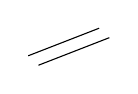
\begin{tikzpicture}[x=1cm,y=1cm]
\draw (0,0)--(0.9,0.35);
\draw (0.13,-0.12)--(1.03,0.23);
\end{tikzpicture}}

Une donnée $(X_i^*)_{i\in I}$ satisfaisant 1°) et 3°) équivaut à
\unsure{une|\deleted{une}} : une relation d'équiv. \uline{loc\textsuperscript{t} finie} et \uline{ouverte}
\deleted{\unsure{telle que les classes soient|telle que les fermés soient}}
et $I$ est l'espace quotient (avec la relation de \inserted{pré}ordre
de spécialisation), \deleted{\illegible{3}} l'ens $I$ est \uline{ordonné} ssi
\[
(\forall i,j\quad\overline{X_i^*}=\overline{X_j^*}\Rightarrow i=j)
\Longleftrightarrow(\text{les }X_i\text{ sont loc. fermés}).
\]

\margin{cas $I$ \uline{ordonné} $\Updownarrow$}
\uline{Stratification} \uline{stricte}

famille loc. finie \inserted{croissante} $(X_i)_{i\in I}$ de fermés, telle que $\forall j<i$
implique que $X_j$ rare dans $X_i$, et $\forall i,j\in I$,
on ait
\[
X_i\cap X_j=\bigcup_{k\in\overline i\cap\overline j}X_k.
\]
\figure{\begin{tikzpicture}\draw (0,0)--(2.4,0);\end{tikzpicture}}

Dans le cadre de la top. modérée, il faut voir comment
\inserted{pour} toute partition par des parties loc. fermées \uline{modérées},
il existe une plus petite \inserted{stratification modérée \unsure{strictes|\deleted{strictes}|\deleted{stricte}}}
\deleted{partition} \unsure{(formée)} \unsure{celles qui|telles que}
\deleted{\unsure{majorent|engendre}} la partition donnée.

% The following line records the ruled division between the two manuscript halves.
\figure{\begin{tikzpicture}\draw (0,0)--(0,-3);\end{tikzpicture}}
\mspage{4)}
\margin{\diagram{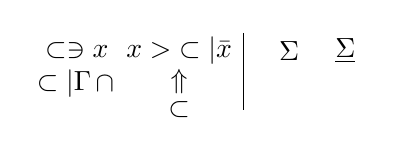
\begin{tikzpicture}[x=0.65cm,y=0.65cm]
\node at (0,0) {$\subset\ni x$};
\node at (2,0) {$x>\unsure{\subset|\bar x}$};
\node at (-0.25,-0.65) {$\unsure{\subset|\Gamma}$};
\node at (0.55,-0.65) {$\unsure{\cap}$};
\node at (2,-0.6) {$\Uparrow$};
\node at (2,-1.15) {$\subset$};
\draw (3.25,0.35)--(3.25,-1.15);
\node at (4.15,0) {$\Sigma$};
\node at (5.25,0) {$\underline{\Sigma}$};
\end{tikzpicture}}}

$(X_i^*)_{i\in I}$ une \inserted{partition indexée} \deleted{famille}
(loc. finie \inserted{de $X$} \deleted{\unsure{de parties disjointes de $X$, de réunion $X$, donc une $X\xrightarrow{\varphi}I$}}). Cond. équiv.

a) $\forall i\in I$, \deleted{\unsure{les $X_i^*\ne\phi$ (i.e. $\varphi$ surj, i.e. une partition), et}}
$\overline{X_i^*}$ est saturé \deleted{\unsure{pour les $X_i^*$ est loc. fermés|pour les $X_i^*$ et loc. fermés}}

b) $\exists\leq$ une \deleted{relation} \inserted{pré}ordre sur $I$, telle que l'on ait $\forall i\in I$
\[
\overline{X_i^*}=\bigcup_{j\leq i}X_j^*
\]
(\unsure{cette|\deleted{cette}} \deleted{relation} préordre est unique, \ldots
\[
i\leq j\Longleftrightarrow\overline{X_i^*}\subset\overline{X_j^*})
\quad(\Longleftrightarrow X_i^*\subset\overline{X_j^*})
\]
c) La top. quotient de $I$ est telle que $\varphi:X\longrightarrow I$ soit ouverte,
i.e. $\forall U\in\operatorname{Ouv}(X)$, le saturé est ouvert

Sous ces conditions, la top. quotient de $I$ est celle
associée à \deleted{\unsure{sa relation d'ordre|la relation d'ordre}} préordre, qui est aussi
la relation de spécialisation pour cette topologie.
Pour que $I$ soit ordonné, il f. et s. que les
$X_i^*$ soient loc\textsuperscript{t}\unsure{.} fermés. On dit alors que la partition est
\uline{stratifiante} \unsure{(i.e. les $X_i^*$ saturés)|\deleted{(i.e. les $X_i^*$ saturés)}}.
\inserted{\unsure{les|\deleted{les}|\illegible{1}} loc. finie, pièces loc. fermées, relation d'équiv. ouverte}

On a une \uuline{correspondance} 1--1 entre les partitions
\inserted{stratifiantes} de $X$ de cette forme, i.e. les relations d'équiv. loc.
finies et ouvertes, \inserted{sur $X$, à fibres loc. fermées}, et l'ens des familles (à iso près)
$(X_i)_{i\in I}$ indexées par un ens. d'indices $I$ \uline{ordonné}
\inserted{\uline{loc. fini}},
qui sont telles que 1°) familles \uline{croissantes} de parties
\inserted{\uline{fermées}} \deleted{\unsure{croissantes}} de $X$, \deleted{\unsure{et}} \uline{recouvrant} $X$, et 2°) $\forall i,j\in I$
\[
X_i\cap X_j=\bigcup_{k\in\overline i\cap\overline j}X_k
\]
\inserted{4°) \deleted{$\unsure{X_\alpha|X_k}$} $\forall i,j\in I$, $j<i$
$\Longrightarrow$ $X_j$ rare dans $X_i$
\unsure{($\forall i,j$, $X_i^*=X_i$)|\deleted{(telle que $X_i^*=X_i$)}}}
\inserted{3°) $\forall i$, $X_i^*\ne\phi$
``déf\unsure{''} $X_i\setminus\bigcup_{j<i}X_j$}

\margin{\uline{NB} Moyennant 1°, 2°, 4°, 3° équivaut à
la cond. plus faible
\unsure{3 bis)|3° bis} $(\forall i\in I)$ $\unsure{X_i|X}\ne\phi$.}

Moyennant 1°) et 2°), en posant $X_i^*=X_i\setminus\bigcup_{j<i}X_j^*$,
les $X_i^*$ forment une ps. partition \inserted{loc. finie} de $X$ par des
ens. loc. fermés, celle-ci satisfait les conditions
d'une \uline{partition} \uline{stratifiante} \uline{stricte} \inserted{avec l'ordre donné de $I$} ssi
on a 3°) et 4°).

\uline{Stratification} : Conditions 1°) et 2°). \uline{Strat. stricte} : ``fidèle'' (i.e.
3°) et condition de densité (4°) : Partitions stratifiantes $\Longleftrightarrow$ strat. strictes
\margin{3}

\scanpage{5}
$\varphi:X\longrightarrow Y$\qquad $\varphi$ ouvert $\overset{\mathrm{déf}}\Longleftrightarrow$ ($U$ ouvert de $X\Rightarrow\varphi(U)$ ouvert)
\[
\Longleftrightarrow\deleted{\unsure{\forall}}\ (\forall B\subset Y,\quad\varphi^{-1}(\overline B)=\overline{\varphi^{-1}(B)})
\qquad(\text{NB }\subset\text{ est l'essentiel})
\]
i.e. $\forall x\in X$, $\varphi(x)\in\overline B\Rightarrow x\in\deleted{\unsure{\varphi^{-1}}}\overline{\varphi^{-1}(B)}$
i.e. $\forall\underset{\mathrm{ouv.}}{U}\ni x$, $U\cap\varphi^{-1}(B)\ne\phi$ i.e.
\[
\forall U\in\operatorname{Ouv}(x),\quad\varphi(U)\cap B\ne\phi
\qquad\text{i.e. }\forall(B\in\mathcal P(Y),x\in X,U\in\operatorname{Ouv}_x(X),)
\]
\[
\varphi(x)\in\overline B\Rightarrow\varphi(U)\cap B\ne\phi\quad\text{i.e.}\quad
\forall(U\in\operatorname{Ouv}(X))\ \forall(y\in\overset{V=}{\varphi(U)},\ B\subset Y),
\]
\[
y\in\overline B\Rightarrow V\cap B\ne\phi\quad\text{i.e.}\quad
\underbrace{V\cap B=\phi}_{B\subset X\setminus V}\Rightarrow\overline B\not\ni y
\]

\par\noindent\rule{0.95\linewidth}{0.4pt}\par

5) Les conditions 1° et 2°) sont stables par image inverse
par $X'\longrightarrow X$, mais pas 3°) bien sûr (pas $=$ pour
un plongement ouvert), ni 4°) (mais au moins
4°) est stable par induction sur un ouvert). Les
relations d'équivalences ouvertes, par contre, s'indui-
sent bien sur un ouvert (mais on rapetisse $I$
en principe). \deleted{Admettons que \unsure{l'on ait pris la même}
\unsure{pour l'un et} 1° 2° (3° bis), \unsure{et alors}\inserted{3° bis} $\forall i,j\in I$, $X_i\subset X_j$
$\Rightarrow i\leq j$}
La condition \inserted{3° bis (en présence de 1° et 2°)}
implique que la ``fidélité'' : $X_i\subset X_j\Rightarrow i\leq j$ (i.e. l'
ordre de $I$ est l'inclusion des $X_i$). \deleted{$I$ \unsure{l'inclusion}}
\deleted{\unsure{Si on a la fidélité, au contraire,} $X_i^*=\phi$ i.e. $X_i=\bigcup_{j<i}X_j$}
n'est pas vrai, exemple $I=$
\diagram{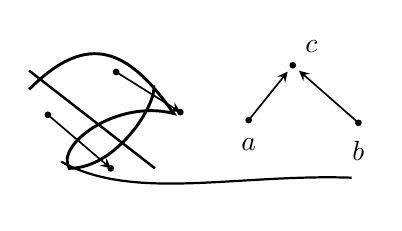
\begin{tikzpicture}[x=1.7cm,y=1.7cm,>=stealth]
\coordinate (dl) at (-1.50,.04);
\coordinate (du) at (-.99,.36);
\coordinate (dr) at (-.51,.06);
\coordinate (dd) at (-1.03,-.36);
\draw[->,line width=.6pt] (dl) -- (dd);
\draw[->,line width=.6pt] (du) -- (dr);
\foreach \p in {dl,du,dr,dd}{\fill (\p) circle (.025);}
\draw[line width=1.05pt] (-1.64,.23) .. controls (-1.19,.68) and (-.89,.52) .. (-.56,.05)
 .. controls (-.99,.16) and (-1.45,-.19) .. (-1.34,-.36)
 .. controls (-.98,-.36) and (-.68,.13) .. (-.71,.26);
\draw[line width=.9pt] (-1.64,.37) -- (-.70,-.36);
\draw[line width=.8pt] (-1.40,-.31) .. controls (-.86,-.61) and (-.09,-.40) .. (.77,-.43);
\coordinate (a) at (0,0);
\coordinate (b) at (.82,-.02);
\coordinate (c) at (.33,.41);
\draw[->,line width=.6pt,shorten >=3pt] (a) -- (c);
\draw[->,line width=.6pt,shorten >=3pt] (b) -- (c);
\foreach \p in {a,b,c}{\fill (\p) circle (.025);}
\node[below=3pt] at (a) {$a$};
\node[below=3pt] at (b) {$b$};
\node[above right=1pt] at (c) {$c$};
\end{tikzpicture}}
$X_c=X=X_a\amalg X_b$, \deleted{\unsure{tous les}} avec $X_a,X_b\ne\phi$, alors \unsure{on a}
fidélité, \inserted{les $X_i\ne\phi$,} mais $X_c^*=\phi$.

On suppose désormais 1°) 2°) 3° bis). Si $U\subset X$
est ouvert, les \inserted{$i\in I$ tels que} $X_i\cap U=U_i$ \deleted{tels que} \inserted{$\ne\phi$} forment un
ouvert $I_U$ de $U$, et \unsure{\deleted{\illegible{1}}|---} $(U_i)_{i\in I_U}$ est une
stratification ps-fidèle de $U$. (Si on part d'une
stratification stricte, on aura une stratification
stricte de $U$). Ainsi, les strat. ps. fidèles des
ouverts de $X$ forment un préfaisceau, dont les
sections sont appelées les stratifications locales
\margin{\unsure{des}}

\deleted{Supposons} \inserted{Soit} $J$ tel que $X_J$ fermé, $J$ non fermé. \inserted{Supposons $J$ minimal}
\deleted{Donc $\exists j\in J$ tel que
$\overline j\not\subset J$. Soit $j$ minimal parmi ces éléments \unsure{de $I$}
$j\in J$, $\overline j\not\subset J$, et $i<j$, $\unsure{\Longleftrightarrow|\Longrightarrow} i\in J\Rightarrow\overline i\subset J$,
\deleted{\unsure{Plus généralement}} \uline{Soit}
\deleted{$\unsure{\overline j\cap J}=\unsure{}% crossed token, no recoverable candidate; crops/150_scan005_P18.png
\unsure{\{j\}}\cup\bigcup i$}
$\unsure{J'_1}=\overline j\cap J$, donc $X_{\unsure{J'_1}}^*=X_{\overline j}^*\cap X_J^*$
est fermé, alors que $J'$ n'est pas fermé. $J'$ \unsure{un}}

parmi de tels $J$ (on suppose $I$ fini, pour simplifier\inserted{$\subset I$}) \unsure{l'on|l'un}
pour tt $K\subset I$, $K$ fermé et $K\cap J$ non fermé, \ldots $K\supset J$.
En particulier, $\forall j\in J$ tel que $\overline j\not\subset J$, \ldots $J\subset\overline j$
i.e. $j$ est plus grand él. de $J$. Donc $J$ a un plus grand
él. $j$, tel que pour tt autre élément \inserted{$j'$} de $J$, on ait
$\overline{j'}\subset J$. Donc \deleted{$\unsure{J}$}
$J_0=J\setminus\{j\}=\bigcup_{j'\in J\setminus\{j\}}\overline{j'}$ est fermé.
Donc $J=J_0\cup\{j\}$, $J_0$ fermé, $\unsure{\exists|\mathrm{et}}$ $J_0\subset\overline j$, $j\in I\setminus J_0$
$\exists i\in I\setminus J_0$ avec $i<j$. \deleted{$i\in\unsure{\overline j\cap I}$} On a donc
\[
X_J^*=X_{J_0}^*\cup X_j^*\quad(\text{réunion disjointe})
\]
qui est fermé, d'où
\[
X_j^\bullet\overset{\mathrm{déf}}=\overline{X_j^*}\setminus X_j^*\subset X_{J_0}^*=X_{J_0}=\deleted{\unsure{\mathrm{ens}}}\bigcup_{i\in J_0}X_i,
\]
sans qu'on ait
pour autant $\overline j\subset J_0\cup\{j\}$.

Soit $I'$ une partie \uline{fermée} de $I$, minimale pour la
propriété : $\exists J\subset I'$, $J$ non fermé, avec $X_J$ fermé. Soit, pour
$I'$ fini, $J$ une \deleted{\unsure{partie}} de $I'$ minimale pour les propriétés précédentes,
On a donc $J\ne\phi$ et $J=J_0\cup\{j\}$, \deleted{$\unsure{\exists}$} $J_0$ fermé, $j\notin J_0$,
\deleted{$\unsure{\overline j\not\ni i}$} $J\subset\overline j$, $\overline j\not\subset J$ \unsure{ceci|ce}, i.e. l'inclusion
\[
J=J_0\cup\{j\}\subset(\overbrace{J_0}^{\subset\overline j}\cup\overline j=\deleted{\unsure{\overline j}}\overline j)
\]
est stricte. \deleted{\unsure{de $I'$}} Pour tte
partie. Comme \inserted{\unsure{tt}} $\overline J\setminus\{j\}$ est encore fermé, d'après la condition
minimale de $I'=\overline J$ il s'ensuit que pour
 tt $J'\unsure{\subset|\in} I'\setminus\deleted{\unsure{\{i\}}}\{j\}$, $X_{J'}^*$ fermé $\Rightarrow J'$ fermé. \deleted{\unsure{En}}

\figure{\begin{tikzpicture}[x=.55cm,y=.55cm]
\foreach \x/\y in {1.87/.61,2.46/.15,2.95/.84,3.54/.96,3.27/-.13,4.10/.51,4.74/1.85,5.79/1.63,5.49/1.34,6.73/2.01,7.77/1.15,7.57/.54,8.66/.93,9.37/.58,9.66/.15,8.92/-.02,9.48/-.13}{\fill (\x,\y) circle (.055);}
\draw[line width=.9pt] (4.10,1.50)
 .. controls (3.98,1.92) and (4.18,2.22) .. (4.70,2.37)
 .. controls (5.40,2.39) and (5.94,2.23) .. (6.33,1.60)
 .. controls (6.41,1.45) and (6.11,1.35) .. (6.13,1.07)
 -- (5.90,1.03)
 .. controls (6.19,.68) and (5.95,.58) .. (5.60,.60)
 -- (5.07,.62)
 .. controls (4.80,.62) and (5.00,.94) .. (4.93,1.13)
 .. controls (4.73,1.30) and (4.33,1.26) .. (4.20,1.34)
 -- cycle;
\node[above right=1pt] at (6.73,2.01) {$j$};
\node at (.80,-.53) {$J_0$};
\end{tikzpicture}}

\deleted{particulier, pour tte partie fermée}
3 conditions équiv. :

a) $X_J^*$ fermé $\Rightarrow J$ fermé

b) $X_L^*$ ouvert $\Rightarrow L$ ouvert

c) $(\underbrace{X_j^\bullet\overset{\mathrm{déf}}=\overline{X_j^*}\setminus X_j^*\subset X_{J_0},\ J_0\text{ fermé}}_{X_{J_0\cup\{j\}}^*\text{ fermé}})
\Rightarrow\overline j\subset J_0\cup\{j\}$
(i.e. $J_0\cup\{j\}$ fermé)
(\uline{NB} \unsure{ssi} $J_0\subset\overline j$), et pour pour
$J'\subset\overline j\setminus\{j\}$, $X_{J'}^*$ fermé $\rightarrow J'$ fermé

\margin{4}

\scanpage{7}
\margin{\unsure{S|5}}

\figure{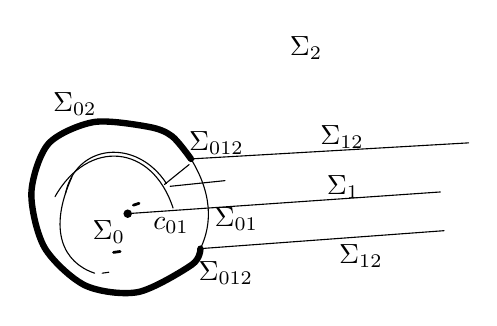
\begin{tikzpicture}[x=0.012cm,y=-0.012cm,line cap=round,line join=round]
\draw[line width=2.3pt] plot[smooth] coordinates {(436,274) (416,250) (391,240) (333,235) (285,258) (267,310) (281,368) (324,408) (380,415) (437,386) (446,369)};
\draw (436,274) .. controls (458,310) and (459,342) .. (446,369);
\draw (303,311) .. controls (314,258) and (378,251) .. (410,300);
\draw (292,314) .. controls (327,252) and (395,258) .. (417,326);
\draw (310,293) .. controls (284,350) and (301,384) .. (334,395);
\draw (342,395)--(349,394);
\draw (414,303)--(472,297) (408,301)--(434,280);
\draw (436,274)--(730,257) (368,332)--(700,309) (446,369)--(704,350);
\draw[line width=1pt] (375,323)--(381,321) (354,373)--(361,372);
\fill (369,332) circle (4.5);
\node at (558,157) {$\Sigma_2$};\node at (313,216) {$\Sigma_{02}$};
\node at (463,257) {$\Sigma_{012}$};\node at (596,251) {$\Sigma_{12}$};
\node at (349,351) {$\Sigma_0$};\node at (415,345) {$c_{01}$};
\node at (484,338) {$\Sigma_{01}$};\node at (597,304) {$\Sigma_1$};
\node at (473,395) {$\Sigma_{012}$};\node at (616,377) {$\Sigma_{12}$};
\end{tikzpicture}}

\margin{$\unsure{\supset d'}$}

\figure{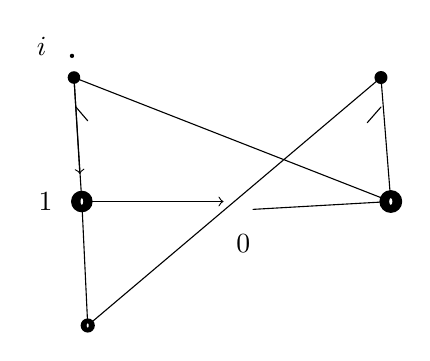
\begin{tikzpicture}[x=0.025cm,y=-0.025cm,line cap=round,line join=round]
\draw (1212,195)--(1373,258)--(1368,195)--(1219,321)--(1216,258);
\draw (1212,195)--(1216,258);
\draw[->] (1212,195)--(1215,244);
\draw[->] (1216,258)--(1288,258);
\draw (1303,262)--(1373,258);
\draw (1213,210)--(1219,217) (1368,210)--(1361,218);
\fill (1212,195) circle (3.2);
\fill (1216,258) circle (5.5);
\fill (1219,321) circle (3.6);
\fill (1368,195) circle (3.3);
\fill (1373,258) circle (5.8);
\fill (1211,184) circle (1.1);
\fill[white] (1216,258) ellipse (0.65 and 1.7);
\fill[white] (1219,321) ellipse (0.5 and 1.1);
\fill[white] (1373,258) ellipse (0.8 and 1.7);
\node[left] at (1203,179) {$\unsure{i}$};
\node[left] at (1206,258) {$1$};\node[below] at (1298,270) {$0$};
\end{tikzpicture}}

$\Sigma_{i_0i_1\ldots i_n}$\qquad\deleted{\unsure{covariant}} foncteur contravariant
par rapport aux drapeaux
variables $(i_0,\unsure{{:}\ldots|i_1\ldots},i_n)$

\[
\Sigma_i=X_i'=X_i\setminus\left(X_i\cap\bigcup_{k<i}\mathop{\overset{\unsure{\bullet|\deleted{\circ}}}{\mathrm{T}}\mathrm{ub}}\nolimits^{\circ}(X_k,X_i)\right)
\]

\[
\Sigma_{(i,j)}=\deleted{\unsure{\partial}}\operatorname{Tub}^{\bullet}\left(X_i',X_j\deleted{\unsure{\varnothing}}\setminus\bigcup_{\substack{\deleted{\unsure{k<j}}\quad\deleted{\unsure{i<k|j<k}}\\\deleted{\unsure{k\ne i}}\\\inserted{i<k<j}}}\operatorname{Tub}(X_k,X_j)\right)\hookrightarrow X_j'=\Sigma_j
\]

\[i<k<j\]

\margin{\diagram{\begin{tikzcd}
\Sigma_\delta\arrow[r,hook]\arrow[d]&\Sigma_{\delta'}\arrow[d]\\
\Sigma_d\arrow[r,hook]&\Sigma_{d'}
\end{tikzcd}}
\diagram{\[\begin{array}{ccc}d&\supset&d'\\&&\cap\\\unsure{\delta|d}&&\delta'\end{array}\]}
cofinaux
\diagram{\begin{tikzcd}\bullet\arrow[d]\\d'\end{tikzcd}}}

\deleted{$\Sigma_{i,j}=T.$}

\diagram{\begin{tikzcd}[column sep=small,row sep=large]
&\mathcal V_{i,j}\arrow[d]&{}=\mathcal V(X_i^*,X_j)\setminus\displaystyle\bigcup_{i\leq k<j}\mathcal V(\unsure{X_i^*|X_i'},X_j)\cap X_k\arrow[r,hook]&X_j^*\\
X&X_i^*&&
\end{tikzcd}}

\noindent $\mathcal V_{ijk}$\par

\diagram{\begin{tikzcd}[row sep=large,column sep=large,execute at end picture={\draw (branchend) ++(0.10,0.13)--(branchend)--++(0.16,-0.03);}]
\mathcal V_{ijk}\arrow[r]\arrow[d]&\mathcal V_{jk}\arrow[d]\arrow[r,hook,no head]&X_k^*\arrow[d,""{name=branch,coordinate,pos=.55}]\\
\mathcal V_{ij}\arrow[r,hook]\arrow[d]&\mathcal V(X_j^*,X_k)\arrow[r,phantom,"\deleted{\xrightarrow{\unsure{\sim}}}" description]&\deleted{X_k}\\
X_i^*&&
\arrow[from=branch,to=2-2,dashed,no head,to path={(\tikztostart)--++(-1.5,-0.45) coordinate (branchend)\tikztonodes},"\unsure{\sim|r}"']
\end{tikzcd}}

\margin{$\lambda_i'\unsure{T'|T^i}=\lambda''T''$\qquad
$a\leq\operatorname{Inf}(\lambda',\lambda_i')$}

\margin{\uline{6}}

\scanpage{8}
$\Sigma_0,\Sigma_1,\Sigma_2$ espaces top.
\[
\Sigma_{01}\subset\Sigma_{01},\quad
\Sigma_{12}\subset\Sigma_1\times\Sigma_2,\quad
\Sigma_{02}\subset\Sigma_0\times\Sigma_2\qquad\text{fermés}
\]
\deleted{\unsure{a)}} Posons
\[
\begin{array}{c@{\;}l}
\Sigma_{012}&\subset\Sigma_0\times\Sigma_1\times\Sigma_2\\
\Vert&\\
(\Sigma_{01}\times\Sigma_2)\cap(\Sigma_0\times\Sigma_{12})&
\end{array}
\]
a) On veut que $\operatorname{Im}(\Sigma_{012}\longrightarrow\Sigma_0\times\Sigma_2)\subset\Sigma_{02}$

de sorte qu'on a un diagramme commutatif
\diagram{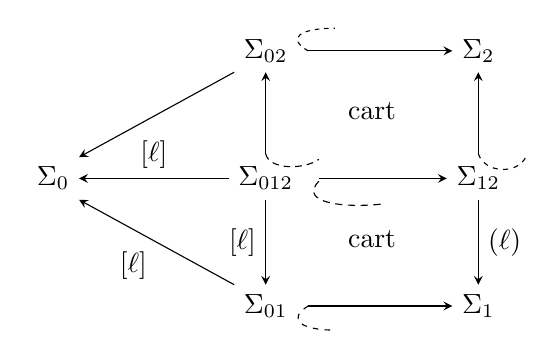
\begin{tikzpicture}[x=1.35cm,y=0.9cm,>=stealth]
\node (S0) at (0,0) {$\Sigma_0$};
\node (S02) at (2,1.8) {$\Sigma_{02}$};
\node (S2) at (4,1.8) {$\Sigma_2$};
\node (S012) at (2,0) {$\Sigma_{012}$};
\node (S12) at (4,0) {$\Sigma_{12}$};
\node (S01) at (2,-1.8) {$\Sigma_{01}$};
\node (S1) at (4,-1.8) {$\Sigma_1$};
\draw[->] (S02.south west)--(S0.north east);
\draw[->] (S012.west)--node[above] {$[\ell]$} (S0.east);
\draw[->] (S01.north west)--node[below left] {$[\ell]$} (S0.south east);
\draw[->] (S012.south)--node[left] {$[\ell]$} (S01.north);
\draw[->] (S12.south)--node[right] {$(\ell)$} (S1.north);
\draw[->] (2.4,1.8)--(S2.west);
\draw[dash pattern=on 1.6pt off 1.8pt] (2.4,1.8) .. controls (2.19,1.98) and (2.32,2.12) .. (2.65,2.12);
\draw[->] (2,0.35)--(S02.south);
\draw[dash pattern=on 2.4pt off 1.8pt] (2,0.35) .. controls (2.03,0.12) and (2.36,0.12) .. (2.5,0.27);
\draw[->] (2.5,0)--(S12.west);
\draw[dash pattern=on 2.6pt off 2pt] (2.5,-0.04) .. controls (2.3,-0.35) and (2.75,-0.42) .. (3.1,-0.36);
\draw[->] (4,0.35)--(S2.south);
\draw[dash pattern=on 1.8pt off 2pt] (4,0.35) .. controls (4.06,0.07) and (4.37,0.05) .. (4.45,0.31);
\draw[->] (2.4,-1.8)--(S1.west);
\draw[dash pattern=on 2pt off 2.3pt] (2.4,-1.8) .. controls (2.2,-1.98) and (2.32,-2.14) .. (2.65,-2.14);
\node at (3,0.95) {\deleted{cart}};
\node at (3,-0.85) {cart};
\end{tikzpicture}}
\margin{signifie que
sur $\Sigma_* = \Sigma_0\amalg\Sigma_1\amalg\Sigma_2$
on a une relation d'ordre
au dessus de $[0,1,2]$}

b) $\Sigma_{01}\longrightarrow\Sigma_1$, $\Sigma_{02}\longrightarrow\Sigma_2$, $\Sigma_{12}\longrightarrow\Sigma_2$ sont injectifs
(et \uline{bordants}) (donc $\Sigma_{012}\longrightarrow\Sigma_{12}$ aussi)
\deleted{\unsure{c)}} \inserted{donc aussi} $\Sigma_{012}\longrightarrow\Sigma_{\unsure{02|\deleted{0}2}}$
\deleted{est injectif} \inserted{et a fortiori}
% Unreadable crossed ink is present above the cancelled equivalence sign; source crop: crops/150_scan008_P07.png.
($\overset{\deleted{\unsure{}}}{\deleted{\unsure{\Longleftrightarrow}}}\;\Sigma_{012}\longrightarrow\Sigma_{02}$).

c) \deleted{est injectif), et \uline{de plus}}
On a $\Sigma_{012}=\Sigma_{02}\cap\Sigma_{12}$ dans $\Sigma_{12}$ i.e.
le carré sup. est aussi cartésien

d) $\Sigma_{12}\longrightarrow\Sigma_1$ est transversal p.r. à
un morphisme bordant $\Sigma_{01}\longrightarrow\Sigma_1$ Cela \unsure{sous que}
$\Sigma_{012}\longrightarrow\Sigma_{12}$ est aussi bordant)

e) $\Sigma_{02}$ et $\Sigma_{12}$ sont \inserted{parties bordantes} transversales dans $\Sigma_2$
(donc $\Sigma_{012}\hookrightarrow\Sigma_{02}$ est aussi bordant)

f) $\Sigma_{01}\xrightarrow{[\mathrm{liss}]}\Sigma_0$, $\Sigma_{02}\longrightarrow\Sigma_0$, $\Sigma_{12}\xrightarrow{(\mathrm{liss}]}\Sigma_1$ fibrant
(donc $\Sigma_{012}\xrightarrow{[\mathrm{liss}]}\Sigma_{02}$ fibrant \deleted{\unsure{donc}} et $\Sigma_{0,12}\xrightarrow{[\mathrm{liss}]}\Sigma_{01}$ aussi)

\margin{(f) devrait se remplacer, par
la condition que le diagramme
\diagram{\begin{tikzcd}\Sigma_{01}&\Sigma_{012}\arrow[l]\arrow[r]&\Sigma_{02}\end{tikzcd}}
au dessus de $\Sigma_0$
est loc\textsuperscript{t} trivial sur $\Sigma_0$.}
\margin{7}

\scanpage{10}
\figure{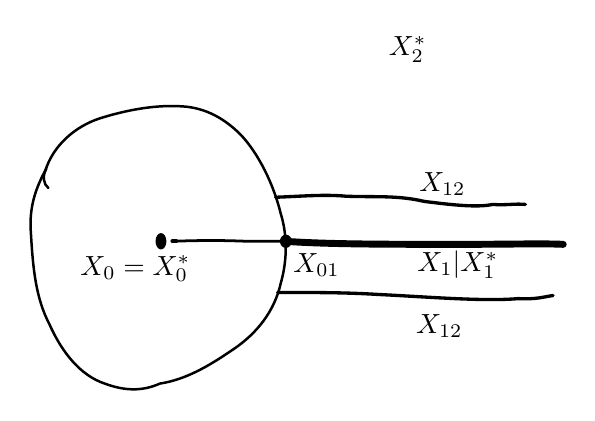
\begin{tikzpicture}[x=0.013cm,y=-0.013cm,line cap=round,line join=round]
\draw[line width=0.9pt]
 (349,190) .. controls (338,210) and (333,229) .. (335,252)
 .. controls (337,287) and (340,315) .. (353,340)
 .. controls (365,367) and (383,390) .. (407,398)
 .. controls (426,405) and (443,406) .. (461,398)
 .. controls (487,394) and (510,380) .. (532,365)
 .. controls (556,349) and (573,327) .. (579,300)
 .. controls (586,276) and (585,251) .. (579,232)
 .. controls (572,203) and (557,173) .. (540,155)
 .. controls (522,137) and (502,127) .. (477,127)
 .. controls (452,126) and (424,132) .. (402,139)
 .. controls (378,147) and (357,165) .. (349,190);
\draw[line width=0.9pt] (350,188) .. controls (346,195) and (347,203) .. (352,207);
\draw[line width=1.2pt]
 (574,216) .. controls (600,215) and (622,213) .. (643,215)
 .. controls (673,216) and (693,214) .. (719,220)
 .. controls (750,224) and (772,226) .. (786,223)
 .. controls (799,224) and (808,222) .. (818,223);
\draw[line width=1.2pt]
 (576,309) .. controls (614,309) and (643,309) .. (675,311)
 .. controls (718,313) and (777,318) .. (811,315)
 .. controls (829,316) and (837,313) .. (845,312);
\draw[line width=1pt]
 (473,259) .. controls (502,258) and (521,258) .. (546,259)
 .. controls (560,259) and (574,259) .. (583,259);
\draw[line width=1.3pt] (473,259)--(477,259);
\draw[line width=2.5pt]
 (583,259) .. controls (625,262) and (687,262) .. (755,262)
 .. controls (801,262) and (836,261) .. (855,262);
\fill (462,259) ellipse [x radius=5.3,y radius=8.0];
\fill (584,259) ellipse [x radius=5.8,y radius=6.5];
\node at (703,72) {$X_2^*$};
\node at (437,286) {$\uline{X}_{\unsure{0}}=\uline{X}_0^*$};
\node at (614,282) {$X_{01}$};
\node at (737,203) {$X_{12}$};
\node at (752,282) {$\unsure{\uline{X}_{\unsure{}1}|\uline{X}_1^*}$};% unrecoverable overtraced group extending above/left of 1; no established cancellation state; crops/150_scan010_P03.png
\node at (734,342) {$X_{12}$};
\end{tikzpicture}}
\margin{\unsure{\uline{9}|9}}

\scanpage{12}
\mspage{1)}
Espaces stratifiés (étude par voisinages \deleted{tubulaires}
\inserted{coniques})
\textcircled{I}

\textcircled{1} Soit $Y$ un espace topologique. Un \uline{voisinage \deleted{tubulaire}} \inserted{\uline{\unsure{conique}}}
\inserted{(``\uline{absolu}'')} de \deleted{$Y$}
\inserted{(ou ``cône sur $Y$'')} est un espace topologique
$T\deleted{\unsure{_Y}}$ contenant $Y$,
(le ``\uline{tube}''), muni d'une partie fermée $\dot T$
\deleted{\illegible{1}} (le ``bord'' du tube'') et d'une opération du monoïde topologique
$\mathbf{I}=[0,1]\,\unsure{}$ (pour la multiplication) sur $T$, notée
% P08: present overworked mark after [0,1]; identity and cancellation state uncertain.
\[
(1)\qquad (\lambda,t)\longmapsto\lambda t
\qquad \mathbf{I}\times T\longrightarrow T
\]
satisfaisant :
\[
\left.\begin{array}{ll}
a)&\lambda y=y\quad\forall y\in Y\\
b)&0.\deleted{\unsure{T|\bar T}}T\subset Y
\end{array}\right\}
\]
\margin{donc les $\lambda_T:T\longrightarrow T$
$(0\leq\lambda\leq1)$ forment une homotopie de
l'identité $\operatorname{id}_T$ (pour $\lambda=1$)
sur une \uline{rétraction} de $T$ sur $Y$,
laissant les pts de $Y$ fixes au cours de l'homotopie}
\margin{\uline{NB} La condition b) sous \unsure{sa|la} forme faible
$0.\dot T\subset Y$, plus la condition c)
(à qui celle-ci donne un sens) suffisent :
entraînent}

c) Le \deleted{application} diagramme d'applications
\diagram{\[
\unsure{(2)|(b)}\qquad
\begin{tikzcd}[column sep=large,
execute at end picture={
\path (p012a.east) -- coordinate[pos=.32] (p012extrahead) (p012b.west);
\draw ([xshift=-3pt,yshift=2pt]p012extrahead) -- (p012extrahead) -- ([xshift=-3pt,yshift=-2pt]p012extrahead);
}]
|[alias=p012a]| \mathbf{I}\times\dot T \arrow[r,"{(\lambda,\unsure{x})\mapsto\lambda x}",
"\deleted{\unsure{g|f}}"'] & |[alias=p012b]| T\\
\{0\}\times\dot T \arrow[u,<->] \arrow[r,"{(0,x)\mapsto0.x}"'] & Y \arrow[u,hook,"\mathrm{inc}"']
\end{tikzcd}
\]}
est \uline{cocartésien}$^{*}$, i.e. identifie $T$ au cône de l'application
\[
(3)\qquad f:\dot T\longrightarrow Y\qquad f(\unsure{a|x})=0.x
\]
\margin{\uline{$^{*}$} Cela signifie que
$\mathbf{I}_{]0,1]}\times\dot T\xrightarrow{\substack{\mathrm{bij.}\\\sim}}T\setminus Y$
et qu'une partie de $T$ est ouverte ssi
\deleted{\unsure{son intersection}} \inserted{\unsure{ses images}}
\unsure{et} \unsure{dans $Y$ et ses images dans $\mathbf{I}\times\dot T$}}
\[
(4)\qquad T\simeq C(f)
\]
Dans cette identification, $Y\hookrightarrow\deleted{\unsure{T}}T
\hookleftarrow\dot T$ correspondent
aux applications canoniques \deleted{\unsure{du cône $f$}}
$\operatorname{but}(f)\hookrightarrow C(f)\hookleftarrow
\operatorname{source}\unsure{(}f\unsure{)}$
et l'opération de $\mathbf{I}$ sur $T$ provient de l'opération de
$\mathbf{I}$ sur $C(f)$, définie par passage au quotient de
l'opération évidente de $\mathbf{I}$ sur $\mathbf{I}\times\dot T$, et l'op. triviale
de $\mathbf{I}$ sur $Y$. Les axiomes a) b) c) signifient
aussi que la situation $(Y\mathrel{\tikz[baseline=-.45ex]{\draw (.12,.09) .. controls (-.01,.09) and (-.01,0) .. (.12,0) -- (.65,0);}}T
\mathrel{\tikz[baseline=-.45ex]{\draw (0,0) -- (.53,0) .. controls (.68,0) and (.68,.11) .. (.53,.13);}}\dot T,
\mathbf{I}\times T-T)$
est isomorphe : celle d'un $C(f)$ avec $f:\dot T-Y$.
Notons que $\dot T$ est connu quand on connaît l'opération
de $\mathbf{I}$ sur $T$, \deleted{\unsure{comme on}} en posant
\[
(5)\qquad \mathring T=T\setminus\dot T
\quad\text{(l'\uline{intérieur} du tube)}
\qquad\text{et notons que }\mathring T=\bigcup_{\lambda\in[0,1[}\lambda T
\]
\margin{11}

\scanpage{13}
\deleted{2. Soit $X$ un espace, $Y$ un sous-espace fermé.}
\unsure{\deleted{(6)}|(6)} \deleted{Soit $T$}

\uline{NB} Les $T_\lambda$ $(\lambda\in[0,1])$ forment
une famille croissante de parties fermées de
$T$, les $\mathring T_\lambda\overset{\mathrm{def}}=
\lambda\mathring T\deleted{\unsure{_\lambda}}$ $(\lambda\in]0,1])$
\margin{$\Vert$}
une famille croissante de parties ouvertes. Si $\lambda\in]0,1[$, alors
$\mathring T_\lambda$ est bel et bien l'intérieur \inserted{topologique}
de $T_\lambda$ dans $T$,
mais bien sûr $\mathring T_1=\mathring T$ n'est pas l'intérieur
\inserted{top.} de $T_1$ dans
l'espace topologique $T_1=T$, i.e. on n'a pas
$\mathring T\unsure{\deleted{_1}|_1}=T$ sauf
si $\dot T=\phi$ i.e. $Y=T$.

Posons, pour $\lambda\in]0,1[$
\[
(\unsure{6})\qquad
\left\{\begin{aligned}
T\setminus\mathring T_\lambda
&\overset{\mathrm{def}}=\deleted{\unsure{E}}
\mathrm{Ep}^{(T)}_{1-\lambda=\varepsilon}
\quad\text{``épaississement d'indice $\varepsilon$''}\\
&\hspace{4em}\text{du bord $\dot T$ de $T$}\\
\dot{\mathrm{Ep}}_\varepsilon^{(T)}
&\overset{\mathrm{déf}}=\dot T\unsure{\amalg|\cup}(1-\varepsilon).\dot T
\end{aligned}\right.
\]
\uline{NB} La frontière de $E_\varepsilon$ dans $T$ est
$(1-\varepsilon)\dot T$, et $E_\varepsilon$
est un voisinage de $\dot T$. On a
\[
(7)\qquad\mathrm{Ep}_\varepsilon^{(T)}
\simeq[\underbrace{1-\varepsilon}_{\lambda},1]\times\dot T
\]
\margin{\uline{NB} Si $Y,\inserted{\dot T}$ compacts, \deleted{\unsure{les}}
alors $T$ compact, et les $T_\varepsilon$
$(\varepsilon\in]0,1])$ forment
un syst. fond. de voisinages de $Y$ dans $T$,
\deleted{\unsure{fermés}}\inserted{ouverts}.
% crops/150_scan013_P07.png: the following live fragment lies below syst. fond.; its attachment is uncertain.
\unsure{plus|plein} : $T$
(\unsure{ainsi que voisinages} tubulaires absolus de $Y$)}
% P07 scope check: the nearby overworked (6) and underlined main-text NB belong to P05/P06, not to this marginal note.

\textcircled{2} Soit $Y\lhook\joinrel\relbar X$ une inclusion fermée d'espaces
 topologiques. Un \uline{voisinage conique} de \uline{$Y$ dans} $X$
est un voisinage $T$ de $Y$ dans $X$
muni d'une opération (1) $I\times T\mathrel{\relbar\joinrel\relbar}T$
\inserted{faisant de $T$ un vois. \deleted{tub.}\inserted{coniq.}
absolu de $Y$.} \deleted{satisfaisant les conditions \unsure{dites.|id.}}
Alors les
$\lambda T=T_\lambda$ $(\lambda\in]0,1])$
forment d'autres voisinages
tubulaires de $Y$ dans $X$ (famille croissante) et
on voit que pour $\lambda\in]0,1[$, on a
\[
(\unsure{8})\qquad\dot T_\lambda=\lambda\dot T
\quad\text{est la frontière de }T_\lambda=\lambda T\text{ dans }X.
\]
\margin{12}

\scanpage{14}
\mspage{2)}
Mais on ne peut pas dire \inserted{en général} que $\dot T$ soit la frontière
de $T$ dans $X$, i.e. (7) devient faux si $\lambda=1$
% P02: crossed group after T; the lambda reading and lowered attachment remain uncertain.
(prendre $X=T\deleted{\unsure{_\lambda}}$, \unsure{pour|avec} $\dot T\neq0$).
% P02: isolated vertical ink point below faux, to the right of the parenthesis; linguistic status unclear.
\figure{\begin{tikzpicture}[x=1cm,y=1cm]
\path[use as bounding box] (0,0) rectangle (10,0.2);
\fill (6.2,0.1) ellipse (0.025 and 0.06);
\end{tikzpicture}}

% P03: the isolated raised capital is not expanded into a word; adjacent slanted ink belongs to the marginal note.
\deleted{\unsure{On dira}} \inserted{\unsure{É|E}} \unsure{enfin de} dire qu'une partie fermée $\deleted{Z}Y$ d'un
espace topologique $X$ est une ``\uline{partie bord}''
s'il existe un \uline{voisinage}-\deleted{\uline{collier}}
% P05: the initial group is overworked; no independent earlier word can be separated from it.
\inserted{\uline{\unsure{c}ylindrique}} de $\deleted{Z}Y$ dans $X$,
i.e. un voisinage \deleted{tubulaire} cônique $T$ tel que
$\dot T\longrightarrow Y$ soit un homéom --- ou ce qui revient
au même, \deleted{\unsure{i.e.} tel que l'on} s'il existe un
voisinage $\deleted{\unsure{de}}T$ de $Y$ dans $X$ et un homéom
\[
(9)\qquad T\simeq Y\times\mathbf{I}
\]
rendant commutatif le diagramme
\diagram{\[
(10)\qquad
\begin{tikzcd}
Y\arrow[r,hook]\arrow[dr,"{y\mapsto(y,0)}"']&T\arrow[d,phantom,"{\wr\!\vert}" description]\\
&Y\times\mathbf{I}
\end{tikzcd}
\]}
\margin{définir la structure de voisinage cylindrique
comme un homéom.
$E\simeq Y\times[0,1]$
compatible avec
% P10: the upper connector has no secure arrowhead; the target is literally [0,1].
\diagram{\[
\begin{tikzcd}[column sep=small,row sep=small]
Y&\unsure{-|\longrightarrow}&[0,1]\\
y&\longmapsto&(y,0)
\end{tikzcd}
\]}}

Par exemple, si $T$ est un voisinage \deleted{tubulaire} cônique
\inserted{(absolu)} de \deleted{\unsure{tout}} $Y$, alors $\dot T$ est un sous-espace bord.
\unsure{donc} $\dot T_\lambda$ est un sous-espace bord de $T_\lambda$ ;
$\deleted{\unsure{\mathrm{Ep}}}\dot T,(1-\unsure{\varepsilon|\delta})\dot T$
et $\dot T\cup(1-\varepsilon)\dot T$ sont des sous-espaces
bords de $\bar{\mathrm{E}}\mathrm{p}_\varepsilon(T)$. \deleted{Dans}
Si $X$ est un espace
\uline{compact}, et $(Y_i)_{i\in I}$ une partie finie de
parties fermées disjointes de $X$, alors
% P14: the lower union index is J-shaped; the I alternative and the contrast with the earlier I remain explicit.
$Y=\bigcup_{i\in\unsure{J|I}}Y_i$ est un sous-espace bord ssi les $Y_i$ le sont
\margin{13}

\scanpage{15}
\deleted{On dit}\inserted{Soit} $T$ un voisinage
\deleted{tubulaire}\inserted{conique} de $Y\subset X$
dans $X$, posons
\[
(11)\qquad X^*=X\setminus\mathring T=(X\setminus T)\cup\dot T
\]
c'est une partie fermée de $X$. \deleted{On dit que}

\uline{Prop\unsure{.}} Conditions équivalentes (où $\lambda\in]0,1[$ donné)

a) $\dot T$ est une partie-bord de $X^*=X\setminus\mathring T$

b) Il existe un homéomorphisme de $X$
avec lui-$=$, transformant $T,\dot T$ en
% crops/150_scan015_P04.png: the crossed lambda-like group may absorb a parenthesis; no separate live opening parenthesis is visible.
$\deleted{\unsure{\lambda}}T_\lambda,\dot T_\lambda)$

b') Comme b, mais en supposant de plus
que l'homéomorphisme induit l'identité
sur $T_{\lambda'}$ (où \deleted{$0<\lambda'<\lambda$}
$\lambda'$ est donné, $0<\lambda'<\lambda$).

c) Il existe un voisinage \deleted{tubulaire} cônique $T'$
de $Y$ dans $X$, \deleted{tel que et \unsure{a}} tel que $T=\lambda T'$,
l'isomorphisme étant compatible avec les
structures de voisinages côniques.

On dit alors que $T$ est un vois. \deleted{tub.} conique
\uline{strict} dans $X$

\margin{Il vaut mieux de definir les voisinages côniques
\unsure{strict|stricts} comme \unsure{des} \uline{germes} de voisinage
plus grand $(1+\varepsilon)T\unsure{-R_{>0}}$
$(\varepsilon>0)$}

\uline{Corollaire} Quand $T$ est vois. \deleted{tub.} con. strict dans $X$,
$\dot T$ est la frontière de $T$ dans $X$.

\uline{Corollaire} Si \deleted{il est}
% crops/150_scan015_P11.png: additional triangular ink has an A-like outline; token/state and possible insertion-caret function remain uncertain.
\unsure{\deleted{$A$}|$A$}\inserted{$T$} voisinage
\deleted{tubulaire}\inserted{conique} de $Y$
dans $X$, les $T_\lambda$ $(\lambda\in]0,1[)$ sont des voisinages
\deleted{tubulaires}\inserted{coniques} stricts
\margin{14}

\scanpage{16}
\mspage{3)}
\textcircled{3} Soit
\deleted{$X\supset Y$, $X$ \unsure{muni de sous-espaces}}
\inserted{$T$ un vois. \deleted{tub.} conique absolu de $Y$.}
% P03: the epsilon-like lowered group is overworked; no independent strike establishes its cancellation state.
\unsure{Soit|Soient} $\unsure{T'_\varepsilon|T'\deleted{_\varepsilon}}\subset T$.
On dit que $T'$ est \uline{sous-espace cônique} dans $T$ si on a
\[
(12)\qquad\left\{\begin{array}{ll}
a)&T'\text{ stable par homothéties }\lambda\in\mathbf{I}\qquad
\deleted{\unsure{\lambda T'\subset T'}}\\
% P04: the initial P has a small raised/retraced remnant, without a recoverable earlier token.
b)&\text{\unsure{Pour} cette opération, }T'\text{ est un voisinage}
\end{array}\right.
\]
\deleted{tubulaire} cônique de $Y$.
\uline{NB} On aura nécessairement $\unsure{\dot T'}=T'\cap\dot T$,
$T'_\lambda=T'\cap T_\lambda$ ;
\deleted{Si $(T_i)_{i\in I}$ est une famille\unsure{,}}
\inserted{la donnée de $T'$ équivaut à}
celle d'un sous-espace fermé $\dot T'$ de $\dot T$
et d'un sous-espace $\unsure{T'|Y'}$ de $Y$, tel que $Y'\supset0.\dot T'$, et,
on a
\[
% P08: separate unrecoverable raised mark above the double-stem I; no established accent meaning or cancellation state.
T'=\operatorname{Im}(\overset{\unsure{}}{\mathbb{I}}\times
\unsure{\dot T'_\lambda|\dot T'\deleted{_\lambda}}
\unsure{\mathrel{\relbar\joinrel\relbar}|\longrightarrow}T)\cup Y'.
\]
\margin{On dit que $T'$ est cônique \uline{strict}
si $T'\cap Y=0.\dot T'$
--- ces $T'$ correspondent donc aux fermés
$\dot T'$ de $\dot T$.}

On dira qu'une structure cônique sur
un $T\supset Y$ est \uline{compatible} avec des sous-espaces
\inserted{fermés} $T_i$ de $T$ $(i\in I)$ si ces derniers
sont côniques pour cette structure.

Soit $T$ un voisinage conique de $Y\subset X$
dans $X$, soit $X'$ \unsure{p}artie fermée de $X$. On
% P11/P12: the apparent mark above the end of compatible belongs to the hooked descender of fermée.
dit que $T$ est \uline{compatible} avec $X'$ si
$X'\cap T$ est cônique dans $T$. On dit qu'il
est \uline{strictement compatible}$^{*}$ avec $T$, si
$T$ est voisinage conique strict, et s'il existe
un voisinage cylindrique de $\dot T$ dans
$X^*=X\setminus\mathring T$, compatible avec
$X'{}^*=X'\cap X^*$,
ou ce qui revient au $=$, s'il existe un
voisinage $E$ de $\dot T$ dans $X^*$, et un iso
\margin{\deleted{\unsure{Définir la notion pour $X'$}}}
\margin{$^{*}$ \deleted{\uline{\unsure{aussi dire}} \uline{\unsure{strict}}}}
\margin{modifier \unsure{sans doute} la définition des
voisinages côniques \unsure{strict|stricts}\ldots}
% P18: one unheaded separator/leader beside the lower marginal note, leaning slightly right down the original page.
\margin{\figure{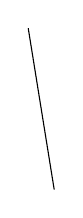
\begin{tikzpicture}[x=1cm,y=1cm]
\draw (0,0)--(0.33,-2.05);
\end{tikzpicture}}}
\margin{15}
